\section{Gaussian Mixture Models}

This section focuses the concept of \acrshort{gmm} for density estimation. For this purpose, the Gaussian normal distribution is presented first, by introducing basic definitions for the probability density functions and describing the closure properties of the distribution. For this purpose, at the beginning a short motivation for the application of the presented model will be given. Then, mixture models in general and \acrshort{gmm} in particular are defined. After that, two main concepts will be explained. First, the \acrshort{gmm} is interpreted in terms of a \acrshort{lvm}. Second, the \acrshort{ema} is presented, which performs the computation of model parameters of latent variable models in an iterative scheme.

\subsection{Gaussian Distribution}

The Gaussian normal distribution forms the basic building block for \acrshort{gmm}s. Depending on the observed random variable, different types of normal distributions exist. In particular, the multivariate normal distribution is focused on when considering statistical flow features, which are typically continuous and high dimensional. In the following, different definitions for the normal distribution are introduced and important properties are presented that are essential for calculations during the learning phase of \acrshort{gmm}s.

Let be a multivariate random variable $\bm{X} = (X_1, \dots, X_D)^T$, where each element $X_d$ with $d \in \{1, \dots, D\}, D \in \mathbb{N}$ is a univariate random variable that follows a normal distribution, which is referred to as $X_d \sim \mathcal{N}(\mu, \sigma^2)$.

\begin{definition}[Univariate Gaussian Distribution] \cite[p. 175]{dei_2020}
A continuous, univariate random variable $X$ is said to follow a normal distribution, if it exhibits a probability density function
\begin{equation*}
p(x | \mu, \sigma^2) = \frac{1}{\sqrt{2\pi \sigma^2}} exp\bigg(- \frac{(x-\mu)^2}{2\sigma^2}\bigg),
\end{equation*}
\end{definition}

with $x \in \mathbb{R}$ and where $\mu$ refers to the mean and $\sigma^2$ is the variance of the distribution. Then, if $\bm{X}$ follows a normal distribution, this is expressed as a multivariate Gaussian distribution, denoted by $\bm{X} \sim \mathcal{N}_D(\bm{\mu}, \bm{\Sigma})$, which is fully described by its mean vector $\bm{\mu}$ and its covariance matrix $\bm{\Sigma}$.

\begin{definition}[Multivariate Gaussian Distribution]\label{def:multivariate_pdf} \cite[175]{dei_2020}
A multivariate random variable $\bm{X}$ follows a normal distribution, if it is described by a probability density function
\begin{equation*}
    p(\bm{x} | \bm{\mu}, \bm{\Sigma}) = (2\pi)^{-\frac{D}{2}} |\bm{\Sigma}|^{-\frac{1}{2}}exp\left(-\frac{1}{2}(\bm{x}-\bm{\mu})^T \bm{\Sigma}^{-1}(\bm{x}-\bm{\mu})\right),
\end{equation*}
\end{definition}

with $\bm{x} \in \mathbb{R}^D$. The mean vector specifies the estimate of the expected value of the distribution, with each of its components describing the mean $\mu$ of the corresponding dimension. The empirical covariance $\bm{\Sigma}$ models the estimate of the variance along each dimension as well as the correlation between the different dimensions. The diagonal elements of $\bm{\Sigma}$ describe the variance of the random variable corresponding to the respective dimension and the off-diagonal elements describe the covariance relationship between the respective random variables. 

An illustration of the influence of the described parameters on the location and shape of a multivariate distribution is given in Figure \ref{fig:multiple_bivariate}. Specifically, three bivariate normal distributions are considered, whose random variables each have different values with respect to their correlation, while the mean vector is the same for all distributions.
 
\begin{figure}%
    \centering%
    \begin{subfigure}[b]{0.25\textwidth}%
        \centering\captionsetup{width=.8\linewidth}%
        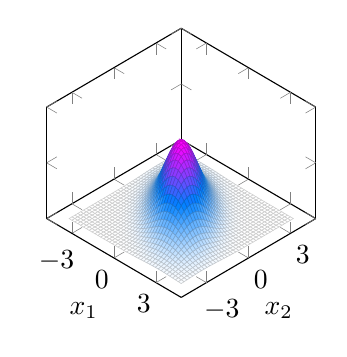
\begin{tikzpicture}
  \def\p{-0.6}%
  \def\centerx{0}%
  \def\centery{0}%
  \pgfplotsset{
      colormap={cool}{rgb255(0cm)=(255,255,255); rgb255(1cm)=(0,128,255); rgb255(2cm)=(255,0,255)}
  }%
    \begin{axis}[
      width=5cm,height=5cm,
      xlabel=$x_1$,
      ylabel=$x_2$,
      xlabel shift={-10pt},
      ylabel shift={-10pt},
      zmin=0,
      zmax=0.2,
      domain=-4:4,
      enlarge x limits,
      enlarge y limits,
      scaled y ticks=false,
      scaled x ticks=false,
      xtick={-3, 0, 3},
      xticklabels={$-3$, $0$, $3$},
      ytick={-3, 0, 3},
      yticklabels={$-3$, $0$, $3$},
      zticklabels={},
      view={45}{45},
      % colorbar horizontal,
      colormap name=cool,
      % colorbar style={
      %   xtick={0, 0.05, 0.1, 0.15, 0.2},
      %   xticklabels={$0$, $0.05$, $0.1$, $0.15$, $0.2$},
      % }
      ]%
      \addplot3[surf, samples=40, shader=faceted, very thin]
      {1/(2 *pi* sqrt(1-\p^2))* exp(-((x-\centerx)^2+(y-\centery)^2-2*\p*(x-\centerx)*(y-\centery))/(2*(1-\p^2))};%
    \end{axis}
\end{tikzpicture}%
        \caption{}%
        \label{subfig:bivariate_neg}%
    \end{subfigure}%
    % \hfill%
    \begin{subfigure}[b]{0.33\textwidth}%
        \centering\captionsetup{width=.8\linewidth}%
        \def\p{0.0}%
\def\centerx{0}%
\def\centery{0}%
\pgfplotsset{
    colormap={cool}{rgb255(0cm)=(255,255,255); rgb255(1cm)=(0,128,255); rgb255(2cm)=(255,0,255)}
}%
\begin{tikzpicture}
    \begin{axis}[
      width=5cm,height=5cm,
      xlabel=$x_1$,
      ylabel=$x_2$,
      xlabel shift={-10pt},
      ylabel shift={-10pt},
      zmin=0,
      zmax=0.2,
      domain=-4:4,
      enlarge x limits,
      enlarge y limits,
      scaled y ticks=false,
      scaled x ticks=false,
      xtick={-3, 0, 3},
      xticklabels={$-3$, $0$, $3$},
      ytick={-3, 0, 3},
      yticklabels={$-3$, $0$, $3$},
      zticklabels={},
      view={45}{45},
      % colorbar horizontal,
      colormap name=cool,
      % colorbar style={
      %   xtick={0, 0.05, 0.1, 0.15, 0.2},
      %   xticklabels={$0$, $0.05$, $0.1$, $0.15$, $0.2$},
      % }
      ]%
      \addplot3[surf, samples=40, shader=faceted,thin]
      {1/(2 *pi* sqrt(1-\p^2))* exp(-((x-\centerx)^2+(y-\centery)^2-2*\p*(x-\centerx)*(y-\centery))/(2*(1-\p^2))};%
    \end{axis}
\end{tikzpicture}%
        \caption{}%
        \label{subfig:bivariate_neutral}%
    \end{subfigure}%
    % \hfill%
    \begin{subfigure}[b]{0.33\textwidth}%
        \centering\captionsetup{width=.8\linewidth}%
        \def\p{0.6}%
\def\centerx{0}%
\def\centery{0}%
\pgfplotsset{
    colormap={cool}{rgb255(0cm)=(255,255,255); rgb255(1cm)=(0,128,255); rgb255(2cm)=(255,0,255)}
}%
\begin{tikzpicture}
    \begin{axis}[
      width=5cm,height=5cm,
      xlabel=$x_1$,
      ylabel=$x_2$,
      xlabel shift={-10pt},
      ylabel shift={-10pt},
      zmin=0,
      zmax=0.2,
      domain=-4:4,
      enlarge x limits,
      enlarge y limits,
      scaled y ticks=false,
      scaled x ticks=false,
      xtick={-3, 0, 3},
      xticklabels={$-3$, $0$, $3$},
      ytick={-3, 0, 3},
      yticklabels={$-3$, $0$, $3$},
      zticklabels={},
      view={45}{45},
      colorbar,
      colormap name=cool,
      colorbar style={
        title={$p(x_1, x_2)$},
        ytick={0, 0.1, 0.197},
        yticklabels={$0.0$, $0.1$, $0.2$},
        height=2.8cm,
        at={(1.1,0)},
        anchor=south west
        % ylabel=$p(x_1, x_2)$
      },
      colorbar/width=2.5mm,
      ]%
      \addplot3[surf, samples=40, shader=faceted,thin]
      {1/(2 *pi* sqrt(1-\p^2))* exp(-((x-\centerx)^2+(y-\centery)^2-2*\p*(x-\centerx)*(y-\centery))/(2*(1-\p^2))};%
    \end{axis}
\end{tikzpicture}%
        \caption{}%
        \label{subfig:bivariate_pos}%
    \end{subfigure}%
    \caption{Bivariate gaussian distributions exhibit different shapes with a changing correlation value between the random variables $x_1$ and $x_2$: (\subref{subfig:bivariate_neg}) negative, (\subref{subfig:bivariate_neutral}) zero and (\subref{subfig:bivariate_pos}) positive correlation}%
    \label{fig:multiple_bivariate}%
\end{figure}%

Having introduced the basic definition of Gaussian distributions, it is now examined how they can be manipulated to obtain information necessary for parameter learning of Gaussian mixture models. Two practical algebraic properties of normal distributions, namely closure under \textit{conditioning} and \textit{marginalization} are detailed for this purpose. Being closed under conditioning and marginalization in this case means that when one or more components of a Gaussian distribution is marginalized out or conditioned on, that the resulting distribution is still Gaussian. This not only distinguishes Gaussian distributions from other distributions, but also makes them easier to handle mathematically. Since both marginalization and conditioning act on subsets of the original distribution, the following notation is introduced first. Considering a multivariate Gaussian random variable $\bm{X} \sim \mathcal{N}(\bm{\mu}, \bm{\Sigma})$, we partition $\bm{X}$ according to 

\begin{equation*}
    \bm{X} = \left[ \begin{array}{c}
        \bm{X}_M \\
        \bm{X}_N
    \end{array} \right],
\end{equation*}

with $\bm{X}_M \in \mathbf{R}^M$, where $M < N$, and $\bm{X}_N \in \mathbf{R}^N$, where $N=D-M$. In general, $\bm{X}_M$ is chosen to be the first $M$ elements of $\bm{X}$ and $\bm{X}_N$ the rest. Accordingly, $\bm{\mu}$ and $\bm{\Sigma}$ are partitioned as
\begin{equation*}
    \left[ \begin{array}{c}
        \bm{X}_M \\
        \bm{X}_N
    \end{array} \right] \sim \mathcal{N} \left( \left[\begin{array}{c}
         \bm{\mu}_M \\
         \bm{\mu}_N
    \end{array}\right], \left[\begin{array}{cc}
        \bm{\Sigma}_{MM} & \bm{\Sigma}_{MN} \\
        \bm{\Sigma}_{NM} & \bm{\Sigma}_{NN}
    \end{array}\right] \right).
\end{equation*}

With this form, it is now possible to express the extraction of partial information from multivariate probability distributions by means of marginalization. 

\begin{definition}[Marginal of a Gaussian Distribution]\label{def:marg_gaussian} \cite[p. 177]{dei_2020}
Given $\bm{X} \sim \mathcal{N}_D(\bm{\mu}, \bm{\Sigma})$, with partitions $\bm{X}_M, \bm{X}_N$, the distributions of $\bm{X}_M$ and $\bm{X}_N$ are called marginals and their corresponding probability density function can be obtained by
\begin{equation*}
    p(\bm{x}_M) = \int p(\bm{x}_M,\bm{x}_N)d\bm{x}_N.
\end{equation*}
\end{definition}

Furthermore, each partition $\bm{X}_M, \bm{X}_N$ only depend on its corresponding entries in $\bm{\mu}$ and  $\bm{\Sigma}$, which leads to the following theorem. 

\begin{theorem} \cite[p. 177]{dei_2020}
The marginal distribution of a Gaussian distribution is also a Gaussian and determined by
\begin{equation*}
    \bm{X}_M \sim \mathcal{N}(\bm{\mu}_M, \bm{\Sigma}_{MM}).
\end{equation*}
\end{theorem}

The conditional Gaussian is typically utilized in the context of posterior distributions, such as in the process of density estimation of \acrshort{gmm}s, and is defined as follows.

\begin{definition}[Conditional of a Gaussian Distribution] \cite[p. 177]{dei_2020}
Given $\bm{X} \sim \mathcal{N}_D(\bm{\mu}, \bm{\Sigma})$, with partitions $\bm{X}_M, \bm{X}_N$, the conditional distribution is defined as
\begin{align*}
    p(\bm{x}_M | \bm{x}_N) &= \mathcal{N}(\bm{\mu}_{M | N}, \bm{\Sigma}_{M | N}), \\
    \bm{\mu}_{M | N} &= \bm{\mu}_M + \bm{\Sigma}_{M N} + \bm{\Sigma}^{-1}_{N N}(\bm{x}_N - \bm{\mu}_N),\\
    \bm{\Sigma}_{M | N} &= \bm{\Sigma}_{M M} - \bm{\Sigma}_{M N} \bm{\Sigma}^{-1}_{N N}\bm{\Sigma}_{N M}.\\
\end{align*}
\end{definition}

\begin{theorem} \cite[p. 177]{dei_2020}
The conditional distribution of a Gaussian distribution is also a Gaussian and defined by 
\begin{equation*}
    \bm{X}_{M | N} \sim \mathcal{N}(\bm{\mu}_{M | N}, \bm{\Sigma}_{M | N}).
\end{equation*}
\end{theorem}

A line of arguments proving the stated theorems can be found in section 2.3 in \cite{bis_2006}.

% \begin{figure}[b]
%     \centering
%     % \documentclass{standalone}

% \usepackage{pgfplots}

% \begin{document}
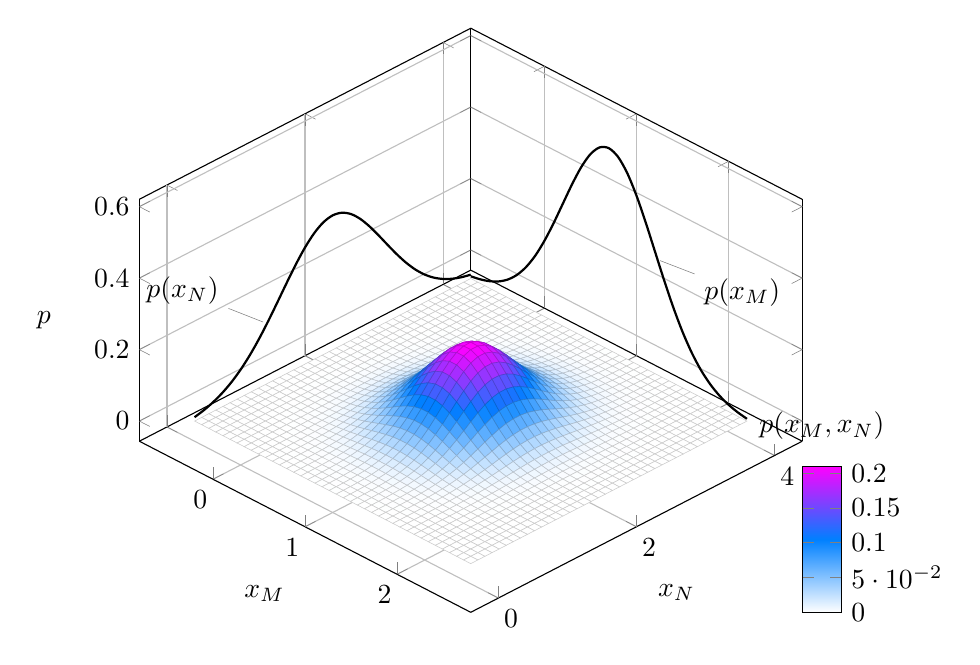
\begin{tikzpicture}[
    declare function={mu1=1;},
    declare function={mu2=2;},
    declare function={sigma1=0.5;},
    declare function={sigma2=0.75;},
    declare function={normal(\m,\s)=1/(2*\s*sqrt(pi))*exp(-(x-\m)^2/(2*\s^2));},
    declare function={bivar(\ma,\sa,\mb,\sb)=
        1/(2*pi*\sa*\sb) * exp(-((x-\ma)^2/\sa^2 + (y-\mb)^2/\sb^2))/2;}]
    \pgfplotsset{colormap={cool}{rgb255(0cm)=(255,255,255); rgb255(1cm)=(0,128,255); rgb255(2cm)=(255,0,255)}}%
\begin{axis}[
    colormap name=cool,
    width=10cm, height=9cm,
    view={45}{45},
    enlarge x limits,
    enlarge y limits,
    grid=major,
    domain=-0.5:2.5,
    y domain=0:4,
    ymin=0,
    ymax=4,
    xmin=-0.5,
    xmax=2.5,
    samples=40,
    xlabel=$x_M$,
    ylabel=$x_N$,
    zlabel={$p$},
    every axis z label/.style={rotate=0, at={(current axis.west)}, left=10mm},
    colorbar,
    colorbar style={
        at={(1,0)},
        anchor=south west,
        height=0.25*\pgfkeysvalueof{/pgfplots/parent axis height},
        title={$p(x_M,x_N)$}
    }
]
\addplot3 [surf, shader=faceted, very thin] {bivar(mu1,sigma1,mu2,sigma2)};
\addplot3 [domain=-0.5:2.5,samples=31, samples y=0, thick, smooth] (x,4,{normal(mu1,sigma1)});
\addplot3 [domain=0:4,samples=31, samples y=0, thick, smooth] (-0.5,x,{normal(mu2,sigma2)});
% \addplot3 [domain=0:4,samples=31, samples y=0, thick, smooth] (x,2,{normal(mu1,0.95)});
\node at (axis cs:-0.4,1,0.18) [pin=165:$p(x_N)$] {};
\node at (axis cs:1.45,4,0.32) [pin=-15:$p(x_M)$] {};
\end{axis}
\end{tikzpicture}
% \end{document}
%     \caption{Cryptographic hash function and locality-sensitive hash function exhibit different properties for the probability of collisions.}
%     \label{fig:hashing_differences}
% \end{figure}

% \begin{figure}[ht!]
% \begin{example}{Examples on the closure properties of Gaussians}{closure_examples}

% Considering the random variable $\bm{X}_a$ from Example \ref{ex:bivariate_gaussian}, the marginalization and conditioning operations are applied and the respective results are visualized . \\

% First, $\bm{X}_a$ is partitioned as
% \begin{equation*}
%     \bm{X}_a = 
%     \left[ \begin{array}{c}
%         X_M \\
%         X_N
%     \end{array} \right] \sim \mathcal{N} \left( \left[\begin{array}{c}
%          0 \\
%          0
%     \end{array}\right], \left[\begin{array}{cc}
%         1.5 & -1.0 \\
%         -1.0 & 0.75
%     \end{array}\right] \right).
% \end{equation*}

% The marginal distributions can be obtained by taking the corresponding values directly from the original distribution, which are
% \begin{align*}
%     p(x_M) = \mathcal{N}(0, 1.5), \\
%     p(x_N) = \mathcal{N}(0, 1.5).
% \end{align*}

% Now, the conditional distribution $p(\bm{x}_M | \bm{x}_N)$ for $\bm{x}_N = 1$ is obtained as
% \begin{align*}
%     \overline{x}_{M | N} &= 0 - 1 + \frac{1}{0.75} \cdot (1-0) = \frac{1}{3}\\
%     \sigma^2_{M | N} &= 1.5 + \frac{1}{0.75} = \frac{17}{6}  \\
%     p(x_{M | N}) &= \mathcal{N}\left(\frac{1}{3} , \frac{17}{6}\right).
% \end{align*}

% \vspace{1cm}

% \begin{minipage}{0.65\textwidth}
%     \centering
%         \begin{subfigure}[t]{\linewidth}
%         \centering
%         \includegraphics[width=0.99\linewidth]{figures/joint_gaussian.png}
%         \subcaption{}
%         \label{fig:joint_gaussian_with_marg}

%         \end{subfigure}
% \end{minipage}
% \begin{minipage}{0.34\textwidth}
%     \centering
%     \begin{subfigure}[t]{\linewidth}
%         %\centering
        
%         \includegraphics[width=0.99\linewidth]{figures/contour_gaussian_conditioned_example.png}
%         \subcaption{}
%         \label{fig:contour_cond_gaussian}
%     \end{subfigure}
%     \begin{subfigure}[t]{\linewidth}
%         %\centering
%         \includegraphics[width=0.99\linewidth]{figures/cond_gaussian.png}
%         \subcaption{}
%         \label{fig:cond_gaussian}
        
%     \end{subfigure}
% \end{minipage}
% \caption[Plots of a joint Gaussian distribution and its corresponding marginal and conditional distributions]{The 3D-plot on the left (\ref{fig:joint_gaussian_with_marg}) shows the joint distribution $p(x_M, x_N)$ with their corresponding marginals. The contour plot on the upper right (\ref{fig:contour_cond_gaussian}) visualizes $p(x_M, x_N)$ with the conditioning value. The plot on the lower right (\ref{fig:cond_gaussian}) illustrates the conditional distribution $p(x_M | x_N)$ with $x_N=1$.}
% \end{example}
% \end{figure}

\newpage
% \input{2_mainmatter/2_theoretical_background/2_2_density_estimation.tex}

\subsection{Gaussian Mixtures}

In this section, the \acrshort{gmm} is presented as a model for density estimation. For this purpose, at the beginning a short motivation for the application of the presented model will be given. Then, mixture models in general and \acrshort{gmm} in particular are defined. After that, two main concepts will be explained. First, the \acrshort{gmm} is interpreted in terms of a \acrshort{lvm}. Second, the \acrshort{ema} is presented, which performs the computation of model parameters of latent variable models in an iterative scheme.

\subsubsection{Motivation}
Using statistical estimation techniques, it is possible to estimate an unobservable underlying probability density function from observed data. This allows data to be compactly represented with a density from a parametric family, such as a Gaussian distribution. However, all conventional parametric distributions are limited in their modeling capabilities when confronted with real data. For example, looking at the marginal distribution $p(x_1)$ in Figure \ref{fig:multimodal_dataset}, it is apparent that the data follow a multimodal distribution, i.e., have more than one center. A density estimate using a simple Gaussian distribution is not sufficient to effectively represent such multimodal data. Therefore, a more flexible type of distribution needs to be introduced that can be used for density estimation.

% \begin{figure}[h]
%     \centering
%     \includegraphics[width=0.8\textwidth]{figures/gaussian_example_dataset.pdf}
%     \caption[Illustration of an exemplary dataset with two dimensions exhibiting a multimodal distribution]{This figure illustrates an examplary dataset with two dimensions. Within the center of this figure, there is a scatter plot showing the observed data points $\bm{x} \in \bm{X}$. At the bottom and right edge of the scatter plot, there are histograms showing the marginal distributions of the dataset.}
%     \label{fig:multimodal_dataset}
% \end{figure}

\subsubsection{Definition}

The idea is to represent a multimodal distribution by constructing a linear combination of multiple simple distributions, each of which representing a unimodal sub-population of the data, which is formalized under the term \textit{mixture model} \cite[p.111]{bis_2006}.

\begin{definition}[Mixture Model] \cite[p. 315]{dei_2020}
A mixture model is a linear combination of $K$ parametric distributions $p_k$, each weighted by a mixture weight $\pi_k$, with the following form 
\begin{align*}
    &p(x) = \sum\limits_{k=1}^K \pi_k p_k (x), \\
    &0 \leq \pi_k \leq 1, \sum\limits_{k=1}^K \pi_k = 1.
\end{align*}
\end{definition}

A distribution $p_k$ within this model is called mixture component and the sum of the mixture weights equals to 1, such that the probability density of the mixture components equals to 1 as well. 

Mixture Models can use any arbitrary parametric distribution as component density, but the most common mixture model is the Gaussian mixture model, using Gaussians as components \cite[214]{has_2009}. First, \acrshort{gmm}s utilize the practical mathematical properties of Gaussians, introduced earlier in Section \ref{sec:gaussian_distribution}. Furthermore, the quality of the model, in terms of its ability to estimate real data distributions, is theoretically supported by the Central Limit Theorem, which states, that most data distributions converge to a normal distribution on average as the number of data points increases (see \cite[p.222]{jay_2003} for a proof).

\begin{theorem}[Central Limit Theorem]\label{th:central_limit} \cite[p.241]{montgomery_2010}
Consider $N$ i.i.d. random variables $X_i$ with $\mathrm{E}[X_i]=\overline{x}$ and $\mathrm{var}[X_i]=\sigma^2$ and let $S_N=\sum^N_{i=1}X_i$. It can be shown that, as $N$ increases, that
\begin{equation*}
    p(S_N) \sim \mathcal{N}\left(\overline{x}, \frac{\sigma^2}{N}\right).
\end{equation*}
\end{theorem}

\begin{definition}[Gaussian Mixture Model]\label{def:gmm} \cite[p. 315]{dei_2020}
A \acrlong{gmm} is a combination of a finite number of $K$ Gaussian distributions $\mathcal{N}(\bm{x}|\theta_k)$ which is fully described by a probability density function $p$ and its parameter set $\theta$ as
\begin{equation}\label{eq:gmm_def}
    \begin{aligned}
        &p(\bm{x}|\theta) = \sum\limits_{k=1}^K \pi_k \mathcal{N}(x | \theta), \\
        &0 \leq \pi_k \leq 1, \sum\limits_{k=1}^K \pi_k = 1, \\
        &\theta := \{\overline{\bm{x}}_k, \bm{\mathrm{C}}_k, \pi_k : k = 1, \dots, K \}.
    \end{aligned}
\end{equation}
\end{definition}

% \begin{figure}[h!]
% \begin{example}{Gaussian Mixture Model with three components}{gmm_examples}

% This example illustrates a \acrshort{gmm} with three components that has been fitted to the dataset shown in Figure \ref{fig:multimodal_dataset}.

% \begin{equation*}
%         p(\bm{x}|\theta) = \sum\limits_{k=1}^{3}\pi_k\mathcal{N}(x|\overline{\bm{x}}_k, \bm{\mathrm{C}}_k)
% \end{equation*}

% \begin{equation*}
% \setlength{\jot}{10pt}
%     \begin{aligned}
%     k = 1:& \quad \pi_1=0.23, \; p_1(\bm{x})=\mathcal{N} \left( \left[\begin{array}{c}
%          3.00 \\
%         -4.68
%     \end{array}\right], \left[\begin{array}{cc}
%         0.57 & -0.41 \\
%         -0.41 & 0.66
%     \end{array}\right] \right)\\
%     k = 2:& \quad  \pi_2=0.33 \; p_2(\bm{x})=\mathcal{N} \left( \left[\begin{array}{c}
%          0.30 \\
%         -6.34
%     \end{array}\right], \left[\begin{array}{cc}
%         0.75 & 0.68 \\
%         0.68 & 1.45
%     \end{array}\right] \right)\\
%     k = 3:& \quad \pi_3=0.44 \; p_3(\bm{x})=\mathcal{N} \left( \left[\begin{array}{c}
%          5.36 \\
%         -5.29
%     \end{array}\right], \left[\begin{array}{cc}
%         0.67 & 0.31 \\
%         0.31 & 0.85
%     \end{array}\right] \right)\\
%     \end{aligned}
% \end{equation*}

%     \begin{subfigure}[ht]{0.66\textwidth}
%         \centering
%         \includegraphics[width=\textwidth]{figures/example_dataset_gmm_3d.png}
%         \caption{}
%         \label{fig:gmm_ex_joint}
%     \end{subfigure}
%     \hfill
%     \begin{subfigure}[ht]{0.33\textwidth}
%         \centering
%         \includegraphics[width=\textwidth]{figures/example_dataset_contour_gmm.png}
%         \caption{}
%         \label{fig:gmm_ex_contour}
%     \end{subfigure}
%     \label{fig:contour_gaussian}
%     \caption[Plots of a Distribution according to a Gaussian Mixture Model]{Both plots visualize a Gaussian Mixture Model that has been fitted to the exemplary dataset from Figure \ref{fig:multimodal_dataset}. Unlike a simple distribution, the mixture model is capable of representing multimodal data.}

% \end{example}
% \end{figure}

\subsubsection{Probabilistic Modeling}
So far, with the definition and the example, an intuitive explanation of the \acrshort{gmm} has been given. Before it is explained how to estimate the parameters of the model, it is necessary to look at the subject from the perspective of probabilistic modeling. Probabilistic models, in general, utilize the mathematics of probability theory in order to express all forms of uncertainty and noise that is associated with the learning task. If a Bayesian interpretation is thereby applied to the probabilities, then this is commonly referred to as Bayesian Inference. This allows, for example, the estimation of the parameters of a probability distribution or a statistical model utilizing Bayes' Theorem \cite[p.245]{dei_2020}. 

In this case, discrete latent variables must be introduced into the construction, which allows a probabilistic model to be formed by defining a joint distribution over observed variables and latent variables \cite[432]{bis_2006}. 

The term latent variable usually refers to a variable that cannot be observed directly, but can be inferred from other observable variables using mathematical models \cite{bor_2003}. Models involving such latent variables, called \acrshort{lvm}, are usually harder to fit than models without latent variables, but often have fewer parameters due to their natural implication of a bottleneck, resulting in a compressed representation of the data \cite[337]{mur_2012}. 

For simplicity, first a single data point $\bm{x}$ is considered, which is later expanded to a set of data points $\bm{X}:=\{\bm{x}_1, \dots, \bm{x}_N\}$. It is further assumed a \acrshort{gmm} with $K$ components. Thus, a $K$-dimensional binary random variable $\bm{z}$ is introduced, that indicates whether the $k$th mixture component is responsible for generating the data point $\bm{x}$. Hence, only a particular element $z_k$ is equal to one and all other elements are equal to zero, such that

\begin{equation}
    z_k \in \{0,1\}, \quad \sum\limits^K_{k=1} z_k=1.
\end{equation}

For the construction of a probabilistic model, it is necessary to specify the joint distribution of the observed data $\bm{x}$ and the latent variable $\bm{z}$. Therefore, the factors of the joint distribution are defined as

\begin{equation}\label{eq:joint_lat_var}
    p(\bm{x},\bm{z}) = p(\bm{z})p(\bm{x}|\bm{z}).
\end{equation}

The responsibility of mixture component $k$ generating a data point $\bm{x}$ can be expressed as the conditional distribution of $\bm{x}$ given a specific assignment for $\bm{z}$, which is a Gaussian

\begin{equation}\label{eq:cond_lat_var}
    p(\bm{x} | z_k=1) = \mathcal{N}(\bm{x} | \overline{\bm{x}}_k, \bm{\mathrm{C}}_k) \quad \Rightarrow \quad p(\bm{x}|\bm{z}) = \prod\limits^K_{k=1}\mathcal{N}(\bm{x} | \overline{\bm{x}}_k, \bm{\mathrm{C}}_k)^{z_k} .
\end{equation}

In practice, there exists no knowledge about the value assignment of the latent variables. Therefore, a prior is set to $\bm{z}$, which is defined as

\begin{equation}\label{eq:prior_lat_var}
    p(\bm{z})=\bm{\pi}=[\pi_{1}, \dots, \pi_{K}]^T = \prod\limits^K_{k=1}\pi_k^{z_k}, \quad \sum\limits_{k=1}^K\pi_{k}=1.
\end{equation}

Now, there is a way to describe the \textit{probability} that the $k$th mixture component generated the data point $\bm{x}$ as

\begin{equation}
    p(z_k=1)=\pi_k.
\end{equation}

% \begin{figure}[h]
%   \begin{minipage}[t]{0.4\textwidth}
%   \vspace{0pt}
%   \centering
%     \caption[A Gaussian Mixture Model represented in plate notation]{
%        Both graphs represent a \acrshort{gmm} using plate notation. While the left graph (a) includes a single data point $\bm{x}$, the graph on the right side (b) extends the model to a full dataset with $N$ i.i.d. data points $\{\bm{x}_n\}$ and corresponding latent variables $\{\bm{z}_n\}$. Note, that the directed edge from the latent variable to the observed data reflects the joint distribution from (\ref{eq:joint_lat_var}).
%     }\label{fig:gmm_plate_notation}
%   \end{minipage}
%   \hfill
%   \begin{minipage}[t]{0.25\textwidth}
%   \vspace{0pt}
%     \begin{tikzpicture}
    \node[obs] (x) {$\bm{x}$};
    \node[latent, above= of x] (z) {$\bm{z}$};
    \node[above=of z] (pi) {$\bm{\pi}$};
    
    \node[left=of x] (cov) {$\bm{\mathrm{C}}_k$};
    \node[above=of cov, yshift=-1cm] (mean) {$\overline{\bm{x}}_k$};
    
    \plate {plate1} {(mean)(cov)} {$k=1, \dots, K$};
    
    \edge{pi}{z};
    \edge{z}{x};
    \edge{mean}{x};
    \edge{cov}{x}
    
    
    \end{tikzpicture}
%     \centering
%     \vspace{2.5pt}
%     (a)
%   \end{minipage}
%   \hfill
%   \begin{minipage}[t]{0.285\textwidth}
%   \vspace{0pt}
%     \subfile{tikz/plate_multi_point.tex}
%     \centering
%     \vspace{2.5pt}
%     (b)
%   \end{minipage}
% \end{figure}

Then the conditional distribution $p(\bm{x}|\bm{z})$ from (\ref{eq:cond_lat_var}) and the prior distribution $p(\bm{z})$ from (\ref{eq:prior_lat_var}) are plugged into the joint distribution $p(\bm{z})p(\bm{x}|\bm{z})$ from (\ref{eq:joint_lat_var}) and the marginal distribution $p(\bm{x})$ is obtained by summing the joint distribution over all possible states of $\bm{z}$, which results in 

\begin{equation}\label{eq:joint_marg_lat_var}
    p(\bm{x}) = \sum\limits_{\bm{z}}p(\bm{z})p(\bm{x}|\bm{z}) = \sum\limits_{k=1}^K\pi_k\mathcal{N}(\bm{x} | \overline{\bm{x}}, \bm{\mathrm{C}}).
\end{equation}

It can be confirmed that the \acrshort{gmm} has been extended by including the discrete latent variable  $\bm{z}$ and that the result is still consistent with the previous definition, since the marginal distribution $p(\bm{x})$ is a Gaussian mixture of the form (\ref{eq:gmm_def}). This enables the joint distribution $p(\bm{x}, \bm{z})$ to be used in place of the marginal distribution $p(\bm{x})$, greatly simplifying parameter estimation by applying the \acrshort{ema}.

So far, it was assumed that the dataset consists of a single data point $\bm{x}$. Now, the dataset is extended to $N$ data points that can be denoted by the matrix $\bm{X} \in \mathbb{R}^{N \times D}$. From that, it follows that every data point $\bm{x}_n$ possesses its own latent variable $\bm{z}_n$. Similarly, all latent variables can be summarized by the matrix $\bm{Z} \in \mathbb{R}^{N \times K}$. This extension to a full dataset is also illustrated comparatively in Figure \ref{fig:gmm_plate_notation}.

In accordance to the full dataset, the corresponding posterior probability after observing $\bm{x}$, referred to as $r_{nk}$, is obtained using Bayes' Theorem as

\begin{equation}\label{eq:responsibilities}
    \begin{aligned}
        r_{nk}=p(z_{nk}=1|\bm{x}_n) &= \frac{p(z_{nk}=1)p(\bm{x} | z_k=1)}{p(\bm{x})}\\[5pt]
        &= \frac{p(\bm{x}_n) | z_{nk}=1)p(z_{nk}=1)}{\sum_{j=1}^K\pi_j p(\bm{x}_n | z_{nj}=1)p(z_{nj}=1)} \\[5pt]
        &= \frac{\pi_k\mathcal{N}(\bm{x}_n) | \overline{\bm{x}}_k, \bm{\mathrm{C}}_k)}{\sum_{j=1}^K\pi_j\mathcal{N}(\bm{x}_n) | \overline{\bm{x}}_j, \bm{\mathrm{C}}_j)}.
    \end{aligned}
\end{equation}

The posterior $r_{nk}$ can be interpreted, from the perspective of a generative model, as the proportion with which a component is involved in the generation of the point $\bm{x}_n$.

\subsubsection{Maximum Likelihood Estimates}

The central question is how to fit the set of unknown parameters $\theta$ to a given set of data $\bm{X}$ and therefore finding a good approximation for the unknown distribution $p(x)$. For estimation problems based on i.i.d. data points, the \acrfull{mle} is an applicable method. \cite[p. 317]{dei_2020} By doing this, the likelihood of each data point $\bm{x} \in \bm{X}$ given a specific parametrization $\theta$ is maximized. 

\newpage

To do so, the likelihood function, and the log-likelihood function respectively, must first be constructed, where each individual likelihood term is a Gaussian mixture density as

\begin{equation*}
    \begin{aligned}
        p(\bm{X}|\theta) &= \prod\limits_{n=1}^Np(\bm{x}_n|\theta), \quad p(\bm{x}_n|\theta)=\sum\limits^K_{k=1}\pi_k\mathcal{N}(\bm{x}_n| \overline{\bm{x}}, \bm{\mathrm{C}}),\\[5pt]
        \mathrm{log}p(\bm{X}|\theta) &= \sum\limits_{n=1}^N \mathrm{log} p(\bm{x}_n|\theta) = \underbrace{ \sum\limits_{n=1}^N \mathrm{log} \sum\limits_{k=1}^K \pi_k \mathcal{N}(\bm{x}_n | \overline{\bm{x}}, \bm{\mathrm{C}})}_{=:\mathcal{L}}.
    \end{aligned}
\end{equation*}

The common solution scheme that would follow would be to calculate the gradient $\partial{\mathcal{L}}/\partial{\theta}$, set it to zero and solve for $\theta$. Unfortunately, there is no closed form solution for a \acrshort{mle} in this form, because the summation over the $K$ components prevents the logarithm from being applied to the Gaussian densities within \cite[p. 435]{bis_2006}. That means that each of the partial derivatives of the model parameters depends on all $K$ parameters of the GMM through $r_{nk}$, which prohibits a closed form solution. 

However, a solution can be found using the \acrshort{ema}. The key idea here is to update one model parameter at a time while keeping the others fixed. For that, the ML estimators for the individual parameters of the \acrshort{gmm} are required first, which will be applied in the \acrshort{ema} in the following step. The following necessary conditions are established:

\begin{equation*}
    \begin{aligned}
    &\frac{\partial{\mathcal{L}}}{\partial{\overline{\bm{x}}_k}} = \bm{0}^T \; &\Longleftrightarrow \quad &\sum\limits_{n=1}^N\frac{\partial{\mathrm{log}p(\bm{x}_n| \theta)}}{\partial{\overline{\bm{x}}_k}} = \bm{0}^T\\[5pt]
    &\frac{\partial{\mathcal{L}}}{\partial{\bm{\mathrm{C}}_k}} = \bm{0} \; &\Longleftrightarrow \quad &\sum\limits_{n=1}^N\frac{\partial{\mathrm{log}p(\bm{x}_n| \theta)}}{\partial{\bm{\mathrm{C}}_k}} = \bm{0}\\[5pt]
    &\frac{\partial{\mathcal{L}}}{\partial{\pi_k}} = 0 \; &\Longleftrightarrow \quad &\sum\limits_{n=1}^N\frac{\partial{\mathrm{log}p(\bm{x}_n| \theta)}}{\partial{\pi_k}} = 0.\\
    \end{aligned}
\end{equation*}

In the following only the partial derivatives of the model parameters that will be used in the \acrshort{ema} are presented. A detailed calculation can be found in \cite[pp.319]{dei_2020}.

\begin{equation}\label{eq:ml_estimator}
    \begin{aligned}
    &\overline{\bm{x}}_k' &= \quad &\frac{\sum_{n=1}^N r_{nk}\bm{x}_n}{\sum_{n=1}^N r_{nk}} \\
    &\bm{\mathrm{C}}_k' &= \quad &\frac{1}{N_k}\sum\limits_{n=1}^N r_{nk}(\bm{x}_n-\overline{\bm{x}}_k)(\bm{x}_n-\overline{\bm{x}}_k)^T\\
    &\pi_k' &= \quad &\frac{N_k}{N}
    \end{aligned}
\end{equation}

\subsubsection{Expectation Maximization Algorithm} \label{ch:Expectation_Maximization_Algorithm}

The \acrshort{ema} is an iterative procedure that starts with an initial estimate of the parameters, which are updated incrementally until convergence is detected. The initial values for the parameters can either be chosen randomly or obtained with an heuristic method, e.g. by using k-means to cluster the data first and subsequently defining the weights based on the resulting k-means memberships \cite[pp. 325]{dei_2020}. 

Each iteration $t$ of the \acrshort{ema} consists mainly of two steps, the Expectation step and the Maximization step. A third step is subsequently needed for the calculation of the convergence criterion. First, in the expectation step, the posterior distribution $r_{nk}$ from (\ref{eq:responsibilities}) is calculated for all data points $\bm{x}_n$ with the current set of parameters $\theta^{(t)}$. Then, the posterior from the previous step is used in the maximization step for computing the new parameter values with the Maximum-Likelihood estimators defined in (\ref{eq:ml_estimator}). At the end of each iteration, the log likelihood for the new set of parameters $\theta^{(t+1)}$ and its change from the log likelihood from the previous iteration is computed. Then, the algorithm can test for convergence by comparing $\Delta \mathcal{L}$ with the convergence threshold $\epsilon$ and the algorithm stops if no significant change occur anymore.

% \begin{algorithm}[H]
% \setstretch{1.75}
% \SetAlgoLined
% \textbf{Initialize:} \;
% $\qquad t=0$\;
% $\qquad \theta^{(t)} := \{\overline{\bm{x}}_k, \bm{\mathrm{C}}_k, \pi_k : k = 1, \dots, K \}$\;
% $\qquad \mathcal{L}^{(t)} = \mathrm{log}p(\bm{X}|\theta^{(t)})$\;
%  \While{$\Delta \mathcal{L} > \epsilon$ }{
%  \BlankLine
% 1. \textit{Expectation-Step:}
% \BlankLine
%     $\qquad r_{nk} = \frac{\pi_k\mathcal{N}(\bm{x}_n | \overline{\bm{x}}_k, \bm{\mathrm{C}}_k)}{\sum_{j=1}^K\pi_j\mathcal{N}(\bm{x}_n) | \overline{\bm{x}}_j, \bm{\mathrm{C}}_j)} \text{ with } \theta^{(t)}$ \;
% \BlankLine
% 2. \textit{Maximization-Step:}
% \BlankLine
% $\qquad \pi_k^{(t+1)} \quad = \frac{N_k}{N}$\;
% $\qquad \overline{\bm{x}}_k^{(t+1)} = \quad \frac{\sum_{n=1}^N r_{nk}\bm{x}_n}{\sum_{n=1}^N r_{nk}}$\;
% $\qquad \bm{\mathrm{C}}_k^{(t+1)} = \quad \frac{1}{N_k}\sum_{n=1}^N r_{nk}(\bm{x}_n-\overline{\bm{x}}_k)(\bm{x}_n-\overline{\bm{x}}_k)^T$\;
% \BlankLine
% 3. \textit{Convergence Terms:}\;
% $\qquad \mathcal{L}^{(t+1)} = \mathrm{log}p(\bm{X}|\theta^{(t+1)})$\;
% $\qquad \Delta \mathcal{L} = | \mathcal{L}^{(t+1)} - \mathcal{L}^{(t)} |$\;
% $\qquad t = t+1$\;
% \BlankLine
%  }
%  \caption{Expectation Maximization for Gaussian Mixture Models}
% \end{algorithm}

Figure \ref{fig:em_algo_gmm} illustrates the EM algorithm for fitting a \acrshort{gmm} with three components to the two-dimensional dataset from Figure \ref{fig:multimodal_dataset}. The resulting \acrshort{gmm} with its component parameters can also be seen in example \ref{ex:gmm_examples}. Each component is represented by an coloured ellipse, that is formed by its mean and covariance matrix. Every single data point $\bm{x}_n$ is associated with an probability vector, that describes each component's responsibility for creating $\bm{x}_n$. This is visualized by coloring each data point according to its probability vector, i.e. a mixed proportion of purple, cyan and orange. At the beginning, the three component parameters are chosen randomly and no posterior $r_{nk}$ is computed yet and thus no data point is colored. With each iteration, the parameters approach the optimum, which they reach after the 21st iteration, and the algorithm converges.

% \begin{figure}[h!]
%     \centering
%     \includegraphics[width=1\textwidth]{figures/em_gaussian.pdf}
%     \caption{Illustration of the EM algorithm for fitting a GMM with three components on a two-dimensional dataset.}
%     \label{fig:em_algo_gmm}
% \end{figure}

How many components should be chosen for fittin a GMM? A common method is to select the model $M$ with the highest probability given the data $D$. Assuming that the model $M$ is completely described by its set of parameters $\theta$, the maximum likelihood function of the model $M$ is given by 

\begin{equation}
    \hat{L} = p(D|\hat{\theta}, M),
\end{equation}
    
answers the question of what is the probability that $D$ is explained by $M$. Note, that the carat denotes the parameters that maximize the probability, i.e., the maximum likelihood function. Theoretically, in the case of a $GMM$, one could just increase the number of parameters $K$, e.g., the number of components, arbitrarily until the $K = N$ in order to obtain the maximum likelihood. In practice, this would not only lead to a bad runtime of the algorithm, but also overfit the model. Thus, the maximum likelihood of the model $L$ has to be balanced against the number of model parameters $K$. The Bayesian information criterion (BIC) is considered as a standard criterion for model selection of GMM because of its theoretical consistency in choosing the number of components \cite{keribin2000consistent}.

In general, the BIC can be defined as

\begin{equation}
    \text{BIC} = K \, \text{ln}(N) - 2 \, \text{ln}(\hat{L}),
\end{equation}

which derives from the findings in \cite{schwarz1978estimating}. The BIC balances the number of model parameters $K$ and number of data points $N$ against the maximum likelihood function $L$. In the model selection, the optimal number of model parameters $K$ minimizes the BIC, such that the BIC provides a principled way of selecting between multiple different models. More complex models almost always fit the data better, resulting in a lower value of $-2 \, \text{ln}(\hat{L})$. The BIC penalizes extra parameters by introducing the term $K \, \text{ln}(N)$. Beyond penalizing more parameters, it furthermore assists in making a judgement as to how the additional parameters improve the model in the presence of more data.

Considering a mixture model with $K$ components defined by 

\begin{equation}
    \begin{aligned}
        &p(\bm{x}|\theta) = \sum\limits_{k=1}^K \pi_k \mathcal{N}(x | \theta), \\
        &0 \leq \pi_k \leq 1, \sum\limits_{k=1}^K \pi_k = 1, \\
        &\theta := \{\overline{\bm{x}}_k, \bm{\mathrm{C}}_k, \pi_k : k = 1, \dots, K \},
    \end{aligned}
\end{equation}

the parameters of $K$ multivariate normal distributions are to learn, with $d$ dimensions, these are $d$ values in the mean vector.  Since a covariance matrix is symmetric, only $d(d+1)/2$ entries in a full covariance matrix have to be computed. Additionaly, $K$ mixture weights have to be determined. Since these sum to one, it is sufficient to determine $K-1$ weights, leading to $Kd + K(d(d+1)/2)+K-1$ parameters. Thus, the BIC for a dataset $D$ with $N$ datapoints of dimensionality $d$ and a GMM $M$ as defined above is stated as 

\begin{equation}
    \text{BIC}(M|D) = (Kd + K(d(d+1)/2)+K-1) \, \text{ln}(N) - 2 \, \text{ln}(\hat{L}).
\end{equation}

A model selection algorithm could look like the following.

\begin{algorithm}
    \caption{GMM Selection with BIC}
    \label{alg:gmm_selection_bic}
    \algsetup{indent=2em}
 
    \begin{algorithmic}[1]
        \REQUIRE Dataset $D$
        \ENSURE Gaussian Mixture Model $M$
        \STATE $B \leftarrow$ new Array
        \STATE GMM $\leftarrow$ new Array
        \FORALL{$k$ in $\{1, \dots, K\}$}
            \STATE $M_k \leftarrow \text{fitGMM}(D)$
            \STATE $b_k \leftarrow \text{BIC}(M|D)$
            \STATE GMM$[k] \leftarrow M_k$
            \STATE $B[k] \leftarrow b_k$
        \ENDFOR
        \STATE $\hat{k} \leftarrow \text{argmin}(B)$
        \STATE $\hat{M} \leftarrow \text{GMM}[\hat{k}]$
        \RETURN $\hat{M}$

        
    \end{algorithmic}
 \end{algorithm}